% Solar Cooker Ray Tracer — Technical Reference
% Compile: pdflatex technical_report.tex  (run twice for ToC)
\documentclass[12pt,a4paper]{report}

% ── Packages ─────────────────────────────────────────────────────────────────
\usepackage[a4paper, margin=2.5cm]{geometry}
\usepackage[T1]{fontenc}
\usepackage[utf8]{inputenc}
\usepackage{lmodern}
\usepackage{microtype}
\usepackage{parskip}
\usepackage{amsmath,amssymb}
\usepackage{booktabs}
\usepackage{float}
\usepackage{caption}
\usepackage{graphicx}
\usepackage{xcolor}
\usepackage{listings}
\usepackage{tikz}
\usetikzlibrary{arrows.meta, positioning, shapes.geometric, fit, backgrounds}
\usepackage{fancyhdr}
\usepackage[hidelinks, colorlinks=true, linkcolor=blue!60!black,
            urlcolor=blue!60!black, citecolor=blue!60!black]{hyperref}

% ── Code listing style ────────────────────────────────────────────────────────
\definecolor{codebg}{HTML}{F5F5F5}
\definecolor{codestring}{HTML}{008000}
\definecolor{codekw}{HTML}{0000CC}
\definecolor{codecomment}{HTML}{808080}

\lstdefinelanguage{json}{
  basicstyle=\ttfamily\small,
  backgroundcolor=\color{codebg},
  frame=single, framerule=0.4pt, rulecolor=\color{gray!40},
  breaklines=true, breakatwhitespace=false,
  columns=fullflexible, keepspaces=true,
  morestring=[b]",
  stringstyle=\color{codestring},
  literate=
    *{0}{{{\color{orange!80!black}0}}}{1}
     {1}{{{\color{orange!80!black}1}}}{1}
     {2}{{{\color{orange!80!black}2}}}{1}
     {3}{{{\color{orange!80!black}3}}}{1}
     {4}{{{\color{orange!80!black}4}}}{1}
     {5}{{{\color{orange!80!black}5}}}{1}
     {6}{{{\color{orange!80!black}6}}}{1}
     {7}{{{\color{orange!80!black}7}}}{1}
     {8}{{{\color{orange!80!black}8}}}{1}
     {9}{{{\color{orange!80!black}9}}}{1}
     {:}{{{\color{black}{:}}}}{1}
     {,}{{{\color{black}{,}}}}{1},
}

\lstdefinestyle{cpp}{
  language=C++,
  basicstyle=\ttfamily\small,
  backgroundcolor=\color{codebg},
  frame=single, framerule=0.4pt, rulecolor=\color{gray!40},
  keywordstyle=\color{codekw}\bfseries,
  commentstyle=\color{codecomment}\itshape,
  stringstyle=\color{codestring},
  breaklines=true, columns=fullflexible, keepspaces=true,
}

\lstdefinestyle{shell}{
  basicstyle=\ttfamily\small,
  backgroundcolor=\color{black!90},
  frame=none,
  breaklines=true, columns=fullflexible, keepspaces=true,
  basicstyle=\ttfamily\small\color{white},
}

% ── Screenshot placeholder macro ─────────────────────────────────────────────
\newcommand{\screenshot}[2][10cm]{%
  \begin{figure}[H]\centering
    \fboxsep=0pt
    \fbox{\begin{minipage}{#1}%
      \centering\vspace{1.8cm}
      \textit{\color{gray}[Screenshot: #2]}
      \vspace{1.8cm}
    \end{minipage}}%
    \caption{#2}%
    \label{fig:\detokenize{#2}}%
  \end{figure}%
}

% ── Headers / footers ─────────────────────────────────────────────────────────
\pagestyle{fancy}
\fancyhf{}
\renewcommand{\headrulewidth}{0.4pt}
\fancyhead[L]{\small\nouppercase{\leftmark}}
\fancyhead[R]{\small Solar Cooker Ray Tracer}
\fancyfoot[C]{\thepage}

% ─────────────────────────────────────────────────────────────────────────────
\begin{document}

% ── Title page ───────────────────────────────────────────────────────────────
\begin{titlepage}
  \centering
  \vspace*{3cm}
  {\Huge\bfseries Solar Cooker Ray Tracer\\[0.6em]}
  {\Large Technical Reference\\[2em]}
  \rule{0.5\textwidth}{0.6pt}\\[2em]
  {\large Version 1.0 \quad|\quad 2026}\\[1em]
  {\normalsize Repository: \texttt{solar-cooker-rt}}\\[3em]
  \vfill
  {\small
    Covers: build system, physics implementation, surface and material models,\\
    Monte Carlo tracer, BVH, GUI navigation, CLI tools, example scenes, and test suite.
  }
\end{titlepage}

% ── Abstract ─────────────────────────────────────────────────────────────────
\chapter*{Abstract}
\addcontentsline{toc}{chapter}{Abstract}

The Solar Cooker Ray Tracer (\texttt{scrt}) is a physically-based Monte Carlo optical
simulator written in C++20.  It models solar concentrating devices—parabolic dishes,
troughs, box cookers, Fresnel lenses, and flat-panel reflectors—by tracing rays from a
realistic sun source through reflective and refractive surfaces onto a receiver, then
computing the spatial flux distribution.

The simulator supports analytic surfaces (paraboloid, plane, sphere, general quadric,
cylindrical paraboloid, Fresnel zone lens) and imported triangle meshes via Assimp.
Materials include perfect mirrors, real mirrors with Gaussian slope error, Beer-Lambert
absorbers, and dielectrics with Fresnel splitting, optional Sellmeier wavelength-dependent
refractive index, and spectrally resolved absorption.  Sun models include a uniform pillbox
and the physically accurate Buie~(2003) circumsolar distribution sampled via tabulated
inverse-CDF.

Tracing is parallelised with \texttt{std::execution::par} over per-thread flux accumulator
buffers.  A Bounding Volume Hierarchy (BVH) with SAH median split accelerates large scenes.
The interactive GUI is built on Polyscope and Dear~ImGui, providing a live 3D view,
per-surface transform sliders, material editing, and a 2D flux heatmap via ImPlot.  A
headless batch mode and a multi-scene comparison driver support automated design sweeps.

\textbf{Intended audience:} engineers and researchers who need to understand, extend, or
validate the simulator.

\tableofcontents

% =============================================================================
\chapter{Project Overview}
% =============================================================================

\section{Purpose}
\texttt{scrt} simulates the optical performance of solar cooker concentrators.  Given a
scene description (sun, reflectors, receiver), it computes the power deposited on the
receiver surface, the peak irradiance, and the concentration ratio—key figures of merit for
solar cooking devices.

\section{Capabilities}
\begin{itemize}
  \item \textbf{Analytic surfaces:} paraboloid, cylindrical paraboloid, plane, sphere,
        general quadric (10-parameter), Fresnel zone lens.
  \item \textbf{Mesh surfaces:} triangulated geometry imported from OBJ, STL, glTF, or FBX
        via Assimp; local per-mesh BVH.
  \item \textbf{Materials:} perfect mirror ($R=1$), real mirror (reflectance + Gaussian slope
        error), dielectric (Fresnel + Beer-Lambert + optional Sellmeier), perfect absorber.
  \item \textbf{Sun models:} uniform pillbox (configurable half-angle) and Buie~2003
        (circumsolar ratio $\chi$).
  \item \textbf{Acceleration:} SAH BVH over the scene graph; O($\log N$) ray queries.
  \item \textbf{Parallelism:} multi-threaded with \texttt{std::execution::par}.
  \item \textbf{Export:} CSV flux map, NumPy \texttt{.npy}, JSON summary, Wavefront OBJ.
  \item \textbf{Interactive GUI:} Polyscope 3D viewer, ImGui panels, ImPlot 2D flux analysis.
\end{itemize}

\section{Operating modes}
\begin{description}
  \item[Interactive (\texttt{scrt\_app})] Opens a Polyscope window.  The user adjusts
    geometry, materials, and sun settings via ImGui sliders, then triggers a trace.
  \item[Headless (\texttt{scrt\_app --headless})] Runs a trace without any display and writes
    results to disk.
  \item[Batch comparison (\texttt{scrt\_compare})] Runs multiple scene files in sequence and
    writes a summary CSV—used in automated design sweeps.
\end{description}

\section{Platform}
Windows~10/11 x64, MSVC v18 (Visual Studio~2025), CMake~4.x, Ninja generator, vcpkg in
manifest mode.  All compiler and SDK paths are encoded in \texttt{CMakePresets.json} so the
build works from any shell without a Developer Command Prompt.

% =============================================================================
\chapter{Build System and Dependencies}
% =============================================================================

\section{Repository layout}

\begin{lstlisting}[language={}, basicstyle=\ttfamily\small, frame=none, backgroundcolor=\color{codebg}]
solar-cooker-rt/
  app/              entry points (main.cpp, compare_main.cpp)
  assets/meshes/    CAD mesh files for import
  docs/             this document, Doxyfile, plan files
  examples/         six JSON scene files
  include/scrt/     public headers (mirrors src/ layout)
    accel/          BVH
    core/           Ray, Hit, AABB, Transform
    io/             SceneLoader, ResultsExporter, MeshImporter
    materials/      Material interface + four implementations
    math/           Vec, Rng, Sampling, Constants
    optics/         Reflect, Refract, Fresnel, Paraxial
    scene/          Scene, Receiver, Aperture
    sources/        SunSource, Pillbox, Buie
    surfaces/       Surface interface + seven implementations
    tracer/         Tracer, FluxAccumulator
    viz/            Viewer, RayRenderer, FluxPlotter
  scripts/          sweep.py, package.ps1
  src/              implementation files (mirrors include/)
  tests/            doctest unit tests
  CMakeLists.txt
  CMakePresets.json
  vcpkg.json
\end{lstlisting}

\section{CMake targets}

\begin{table}[H]\centering
\caption{CMake build targets}
\begin{tabular}{llp{7cm}}
\toprule
Target & Type & Purpose \\
\midrule
\texttt{scrt\_core} & Static lib & Physics engine—all optics, surfaces, materials, tracer.  No GUI dependency. \\
\texttt{scrt\_viz}  & Static lib & Polyscope / ImGui / ImPlot GUI layer. \\
\texttt{scrt\_app}  & Executable & Interactive viewer + headless CLI (\texttt{app/main.cpp}). \\
\texttt{scrt\_compare} & Executable & Headless batch comparison (\texttt{app/compare\_main.cpp}). \\
\texttt{scrt\_tests}   & Executable & doctest unit test suite (\texttt{tests/}). \\
\texttt{docs}          & Custom & Doxygen HTML generation (optional). \\
\bottomrule
\end{tabular}
\end{table}

\section{External libraries}

\begin{table}[H]\centering
\caption{Third-party libraries}
\begin{tabular}{llll}
\toprule
Library & Version & Obtained via & Purpose \\
\midrule
GLM              & vcpkg baseline & vcpkg        & \texttt{dvec3}/\texttt{dmat4} math \\
nlohmann-json    & vcpkg baseline & vcpkg        & JSON scene parsing \\
Assimp           & v6.0.4         & vcpkg        & Mesh import (OBJ/STL/glTF/FBX) \\
doctest          & vcpkg baseline & vcpkg        & Unit testing framework \\
fmt              & vcpkg baseline & vcpkg        & Formatted string output \\
spdlog           & vcpkg baseline & vcpkg        & Structured runtime logging \\
Polyscope        & v2.3.0         & FetchContent & 3D visualisation window \\
Dear ImGui       & (via Polyscope)& Polyscope bundle & UI widgets \\
ImPlot           & v0.17          & FetchContent & 2D flux heatmaps \\
\bottomrule
\end{tabular}
\end{table}

\noindent\textbf{Note on Polyscope:} Polyscope v2.3.0 is not in the vcpkg registry and is
fetched via CMake \texttt{FetchContent} at configure time.  It bundles an older version of
GLM (pre-1.0) whose \texttt{dual\_quaternion} extension is incompatible with the vcpkg GLM
1.0+ headers, so Polyscope's include path is prepended to resolve the conflict.

\section{Build presets}

\begin{table}[H]\centering
\caption{CMakePresets.json configure presets}
\begin{tabular}{llll}
\toprule
Preset & Build type & Triplet & MSVC runtime \\
\midrule
\texttt{debug}        & Debug   & \texttt{x64-windows}        & /MDd (dynamic) \\
\texttt{release}      & Release & \texttt{x64-windows}        & /MD  (dynamic) \\
\texttt{release-dist} & Release & \texttt{x64-windows-static} & /MT  (static)  \\
\bottomrule
\end{tabular}
\end{table}

The \texttt{release-dist} preset statically links every vcpkg package and the MSVC
runtime, producing self-contained executables with zero DLL dependencies.

\section{Building from source}

\begin{lstlisting}[style=shell]
# Configure (first run downloads Polyscope + builds vcpkg deps; ~10-30 min)
cmake --preset debug

# Build all targets
cmake --build --preset debug --parallel

# Run tests
ctest --test-dir build/debug --output-on-failure

# Release distributable (static link)
cmake --preset release-dist
cmake --build --preset release-dist --target scrt_app scrt_compare
\end{lstlisting}

% =============================================================================
\chapter{Software Architecture}
% =============================================================================

\section{Module dependency diagram}

\begin{figure}[H]\centering
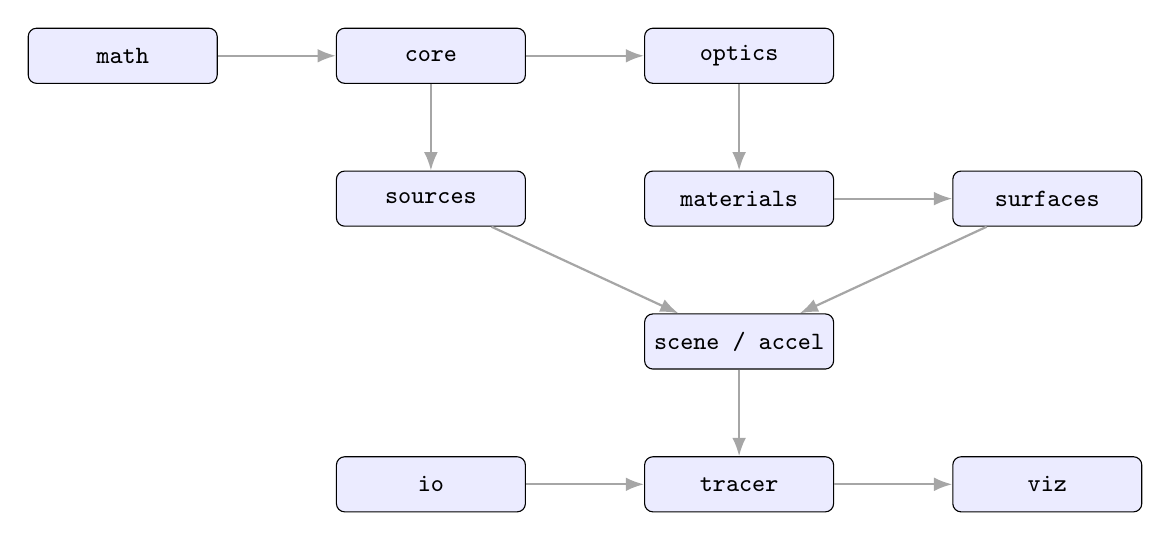
\begin{tikzpicture}[
  node distance=1.1cm and 1.5cm,
  box/.style={draw, rounded corners=3pt, fill=blue!8, minimum width=2.4cm,
              minimum height=0.7cm, font=\small\ttfamily, align=center},
  arr/.style={-Latex, gray!70, thick},
]
  \node[box] (math)    {math};
  \node[box, right=of math] (core)    {core};
  \node[box, right=of core] (optics)  {optics};
  \node[box, below=of core] (sources) {sources};
  \node[box, right=of sources] (mats) {materials};
  \node[box, right=of mats]   (surfs) {surfaces};
  \node[box, below=of mats]   (scene) {scene / accel};
  \node[box, below=of scene]  (tracer){tracer};
  \node[box, left=of tracer]  (io)    {io};
  \node[box, right=of tracer] (viz)   {viz};

  \draw[arr] (math)   -- (core);
  \draw[arr] (core)   -- (optics);
  \draw[arr] (core)   -- (sources);
  \draw[arr] (optics) -- (mats);
  \draw[arr] (mats)   -- (surfs);
  \draw[arr] (surfs)  -- (scene);
  \draw[arr] (sources)-- (scene);
  \draw[arr] (scene)  -- (tracer);
  \draw[arr] (io)     -- (tracer);
  \draw[arr] (tracer) -- (viz);
\end{tikzpicture}
\caption{Module dependency graph (arrow = depends on)}
\end{figure}

\section{Coordinate system and conventions}

\begin{itemize}
  \item Right-handed world coordinate system; $+z$ points upward in typical scenes.
  \item SI units throughout: metres, watts, radians.  Nanometres are used only at I/O
        boundaries (wavelength JSON field; Sellmeier formula input).
  \item All geometry and physics use \texttt{double} precision (\texttt{glm::dvec3},
        \texttt{glm::dmat4}).  No custom vector type is defined; GLM aliases are used.
  \item Every surface is defined in its own canonical local frame and placed in the world
        via an affine \texttt{Transform}.  Intersections are solved in local space and
        results transformed back.
\end{itemize}

\section{Data flow}

A simulation run proceeds as follows:

\begin{enumerate}
  \item \texttt{SceneLoader} parses the JSON file into a \texttt{Scene} object containing
        materials, surfaces, receiver, aperture, and sun source.
  \item \texttt{Scene::build\_acceleration\_structure()} constructs the BVH over all surfaces.
  \item \texttt{Tracer::run()} spawns worker threads.  Each thread samples primary rays from
        the aperture, bounces them through the scene, and deposits absorbed power into a
        per-thread \texttt{FluxAccumulator}.
  \item Thread accumulators are merged and \texttt{finalize()} converts accumulated power to
        flux (W/m$^2$) by dividing each bin by its area.
  \item \texttt{ResultsExporter} writes CSV, NumPy, and JSON outputs.  The interactive GUI
        reads the accumulator to update the Polyscope receiver mesh and the ImPlot heatmap.
\end{enumerate}

% =============================================================================
\chapter{Core Data Structures}
% =============================================================================

\section{Ray}

A \texttt{Ray} carries optical energy through the scene.

\begin{table}[H]\centering
\caption{Ray fields}
\begin{tabular}{lll}
\toprule
Field & Type & Meaning \\
\midrule
\texttt{origin}         & \texttt{dvec3}   & World-space starting point \\
\texttt{direction}      & \texttt{dvec3}   & Unit propagation direction \\
\texttt{power}          & \texttt{double}  & Optical power carried (W) \\
\texttt{wavelength\_nm} & \texttt{double}  & Wavelength in nm (for dispersion) \\
\texttt{bounces}        & \texttt{int}     & Number of bounces so far \\
\texttt{id}             & \texttt{uint32}  & Unique index within the trace run \\
\bottomrule
\end{tabular}
\end{table}

Each primary ray is assigned a power of $P_{\text{ray}} = \text{DNI} \times A_{\text{aperture}} / N_{\text{rays}}$,
so the sum over all rays that hit the receiver converges to the total absorbed power.

\section{Hit}

A \texttt{Hit} record is populated by \texttt{Surface::intersect} and consumed by
\texttt{Material::interact} and \texttt{FluxAccumulator::deposit}.

\begin{table}[H]\centering
\caption{Hit fields}
\begin{tabular}{lll}
\toprule
Field & Type & Meaning \\
\midrule
\texttt{t}          & \texttt{double}   & Parametric distance along ray \\
\texttt{position}   & \texttt{dvec3}    & World-space intersection point \\
\texttt{normal}     & \texttt{dvec3}    & Outward unit normal (against incoming ray) \\
\texttt{uv}         & \texttt{dvec2}    & Surface parametric coords $\in [-1,1]^2$ for flux mapping \\
\texttt{front\_face}& \texttt{bool}     & True when hitting the outer face (entering medium) \\
\texttt{surface}    & \texttt{Surface*} & Pointer to the intersected surface (for material lookup) \\
\bottomrule
\end{tabular}
\end{table}

\section{AABB}

An axis-aligned bounding box used for BVH construction and ray culling.  Key operations:

\begin{itemize}
  \item \texttt{expand(point)} / \texttt{expand(AABB)} — grow to enclose a point or box.
  \item \texttt{intersect(ray, t\_near, t\_far)} — slab-method test; returns false if the ray
        misses the box entirely.
  \item \texttt{centroid()} — geometric centre, used for BVH split decisions.
\end{itemize}

\section{Transform}

An affine transformation storing a $4\times4$ matrix and its precomputed inverse.

\begin{itemize}
  \item Named constructors: \texttt{from\_translation}, \texttt{from\_euler\_xyz},
        \texttt{from\_rotation\_axis\_angle}, \texttt{from\_look\_at}.
  \item \texttt{compose(child)}: returns a transform that applies \texttt{child} first, then
        \texttt{self}.  Used to chain base $\times$ delta transforms in the viewer.
  \item \texttt{normal\_to\_world(n)}: transforms surface normals using the inverse-transpose
        of the matrix, which is correct under non-uniform scale.
  \item \texttt{ray\_to\_local(ray)}: converts a world-space ray to the surface's local frame
        so intersection equations can be solved in canonical coordinates.
\end{itemize}

% =============================================================================
\chapter{Optical Physics}
% =============================================================================

\section{Reflection}

The specular reflection direction is:
\begin{equation}
  \mathbf{r} = \mathbf{d} - 2\,(\mathbf{d}\cdot\hat{\mathbf{n}})\,\hat{\mathbf{n}}
\end{equation}
where $\mathbf{d}$ is the incident (unit) direction and $\hat{\mathbf{n}}$ is the outward
surface normal, oriented so that $\mathbf{d}\cdot\hat{\mathbf{n}} < 0$.

\section{Snell's Law / Refraction}

\begin{equation}
  n_1 \sin\theta_i = n_2 \sin\theta_t
\end{equation}

The vector form used in \texttt{refract(i, n, eta)} with $\eta = n_1/n_2$ is:
\begin{equation}
  \mathbf{t} = \eta\,\mathbf{i} + \left(\eta\cos\theta_i - \cos\theta_t\right)\hat{\mathbf{n}}
\end{equation}

If $\sin^2\theta_t = 1 - \eta^2(1 - \cos^2\theta_i) > 1$, the refracted angle is undefined
and \emph{total internal reflection} (TIR) occurs; the ray is reflected instead.

\section{Fresnel Equations (unpolarised)}

For a ray travelling from medium $n_1$ to $n_2$ at angle of incidence $\theta_i$:
\begin{align}
  R_s &= \left(\frac{n_1\cos\theta_i - n_2\cos\theta_t}{n_1\cos\theta_i + n_2\cos\theta_t}\right)^2 \\[4pt]
  R_p &= \left(\frac{n_2\cos\theta_i - n_1\cos\theta_t}{n_2\cos\theta_i + n_1\cos\theta_t}\right)^2 \\[4pt]
  R   &= \tfrac{1}{2}(R_s + R_p), \qquad T = 1 - R
\end{align}

A Schlick approximation is also available for performance-critical paths:
\begin{equation}
  R(\theta) \approx R_0 + (1-R_0)(1 - \cos\theta)^5, \qquad
  R_0 = \left(\frac{n_1-n_2}{n_1+n_2}\right)^2
\end{equation}

\section{Beer-Lambert Absorption}

Optical power attenuates exponentially inside an absorbing medium:
\begin{equation}
  P_{\text{out}} = P_{\text{in}}\, e^{-\alpha\, d}
\end{equation}
where $\alpha$ (m$^{-1}$) is the absorption coefficient and $d$ is the path length through
the medium.  In the \texttt{Dielectric} material the transmitted ray power is scaled by this
factor using the $t$ parameter of the \texttt{Hit} record.

\section{Sellmeier Dispersion}

Wavelength-dependent refractive index (used when \texttt{"sellmeier"} is set in the scene
JSON):
\begin{equation}
  n^2(\lambda) = 1 + \sum_{i=1}^{3} \frac{B_i\,\lambda^2}{\lambda^2 - C_i}
\end{equation}
$\lambda$ is in micrometres; $C_i$ are the resonance wavelengths squared.  Built-in presets:

\begin{table}[H]\centering
\caption{Sellmeier coefficients for built-in glass presets}
\begin{tabular}{lcccccc}
\toprule
Preset & $B_1$ & $B_2$ & $B_3$ & $C_1$ & $C_2$ & $C_3$ \\
\midrule
N-BK7 borosilicate & 1.03961 & 0.23179 & 1.01047 & 0.00600 & 0.02001 & 103.560 \\
Fused silica        & 0.69617 & 0.40794 & 0.89748 & 0.00468 & 0.01351 & 97.934  \\
\bottomrule
\end{tabular}
\end{table}

\section{Buie Sunshape}

Based on Buie~et~al.\ (2003), the solar radiance profile is parameterised by the
circumsolar ratio $\chi \in [0.02, 0.10]$ (a typical clear-sky value is $\chi = 0.05$).

Shape parameters derived from $\chi$:
\begin{align}
  \kappa &= 0.9\,\ln(13.5\chi)\,\chi^{-0.3} \\
  \gamma &= 2.2\,\ln(0.52\chi)\,\chi^{0.43} - 0.1
\end{align}

Normalised radiance profile:
\begin{equation}
  I(\theta) = \begin{cases}
    \dfrac{\cos(0.326\,\theta)}{\cos(0.308\,\theta)} & \theta \leq 4.65\;\text{mrad} \\[8pt]
    e^\kappa \cdot \theta^\gamma & \theta > 4.65\;\text{mrad}
  \end{cases}
\end{equation}

Rays are sampled from the inverse-CDF of the solid-angle-weighted distribution
$f(\theta)\sin\theta$, tabulated at 4096 bins over $[0,\;43.6\;\text{mrad}]$.  The azimuth
$\phi$ is drawn uniformly from $[0, 2\pi)$.

\section{Surface slope error}

A \texttt{RealMirror} perturbs the surface normal before reflection:
\begin{equation}
  \hat{\mathbf{n}}' = \mathrm{normalize}\!\left(\hat{\mathbf{n}} + \sigma_s\,\boldsymbol{\varepsilon}\right),
  \qquad \boldsymbol{\varepsilon} \sim \mathcal{N}(0,1)^2 \;\text{in the tangent plane}
\end{equation}
where $\sigma_s$ is the 1-$\sigma$ slope error in milliradians.  This models manufacturing
roughness and mirror alignment errors.

% =============================================================================
\chapter{Surface Types}
% =============================================================================

Every surface stores an affine \texttt{Transform}.  Intersection is solved in the canonical
local frame, then the hit position, normal, and UV are transformed back to world space.

\section{Plane}

Canonical equation: $z = 0$, clipped to $[-h_w, h_w]\times[-h_h, h_h]$.

Intersection: $t = -\mathbf{o}_z / \mathbf{d}_z$.  The hit UV coordinates map directly to
the rectangle: $u = x/h_w$, $v = y/h_h$.  Used for flat reflectors, the receiver surface,
and box-cooker panels.

\section{Paraboloid}

Canonical equation: $x^2 + y^2 = 4fz$, with focus at $(0,0,f)$ and aperture circle of
radius $r_a$.

Substituting the ray $\mathbf{p}(t) = \mathbf{o} + t\mathbf{d}$ gives the quadratic:
\begin{equation}
  (d_x^2 + d_y^2)\,t^2 + 2(o_x d_x + o_y d_y - 2f\,d_z)\,t + (o_x^2 + o_y^2 - 4f\,o_z) = 0
\end{equation}

The smallest positive root within the aperture circle is selected.  Normal: $\nabla F =
(2x, 2y, -4f)$ normalised.

\section{Cylindrical Paraboloid}

Canonical equation: $x^2 = 4fz$, extruded in $y$.  Focal line at $(0, y, f)$ for all $y$.

Used for parabolic trough concentrators.  The quadratic degenerates to a problem in $x$ and
$z$ only, with $y$ unbounded (clipped by \texttt{aperture\_half\_length\_m}).

\section{Sphere}

$|\mathbf{p} - \mathbf{c}|^2 = R^2$.  Standard quadratic solve.  Used in tests and as a
secondary optical element.

\section{General Quadric}

Ten-parameter implicit surface:
\begin{equation}
  Ax^2 + By^2 + Cz^2 + Dxy + Exz + Fyz + Gx + Hy + Iz + J = 0
\end{equation}
clipped to an axis-aligned bounding box (\texttt{aperture\_box}).  Substituting the ray
parametrically gives a quadratic in $t$.  The gradient $\nabla F = (2Ax + Dy + Ez + G,
\ldots)$ gives the normal.  Used for the Scheffler off-axis dish (\texttt{scheffler\_reflector.json}).

\section{Fresnel Zone Lens}

A flat disc ($z=0$) divided into $N$ concentric annular zones, each with precomputed facet
tilt angle $\alpha_i$ so that a paraxial ray at ring $i$ is refracted toward the focal point
$(0,0,-f)$.  Paired with a \texttt{Dielectric} material (\texttt{n\_lens}).

JSON parameters: \texttt{focal\_length\_m}, \texttt{inner\_radius\_m}, \texttt{pitch\_m},
\texttt{n\_zones}, \texttt{n\_lens}.

\section{Triangle Mesh}

Arbitrary geometry imported from OBJ/STL/glTF/FBX via Assimp.  A local BVH (SAH median
split over individual triangles) accelerates per-mesh ray queries.  Each triangle is tested
with the Möller--Trumbore algorithm.  Useful for complex housings, non-standard receivers,
or imported CAD parts.

\section{Surface parameter reference}

\begin{table}[H]\centering
\caption{JSON surface types and required parameters}
\begin{tabular}{lll}
\toprule
JSON \texttt{"type"} & Required parameters & Typical use \\
\midrule
\texttt{plane}                  & \texttt{half\_width}, \texttt{half\_height} & Flat reflector, receiver \\
\texttt{paraboloid}             & \texttt{focal\_length\_m}, \texttt{aperture\_radius\_m} & Dish concentrator \\
\texttt{cylindrical\_paraboloid}& \texttt{focal\_length\_m}, \texttt{aperture\_half\_width\_m},
                                  \texttt{aperture\_half\_length\_m} & Trough \\
\texttt{sphere}                 & \texttt{radius} & Curved element \\
\texttt{quadric}                & \texttt{coeffs} \{A--J\}, \texttt{aperture\_box} \{min,max\} & Scheffler dish \\
\texttt{fresnel\_zone\_lens}    & \texttt{focal\_length\_m}, \texttt{inner\_radius\_m},
                                  \texttt{pitch\_m}, \texttt{n\_zones}, \texttt{n\_lens} & Flat lens \\
\texttt{mesh}                   & \texttt{path}, \texttt{scale\_to\_meters} & Imported CAD geometry \\
\bottomrule
\end{tabular}
\end{table}

% =============================================================================
\chapter{Material Models}
% =============================================================================

\section{PerfectMirror}

$R = 1.0$, no power loss.  Returns the reflected ray direction; power is unchanged.
Useful as an ideal upper bound during design.

\section{RealMirror}

Parameters: \texttt{reflectance} $\rho \in [0,1]$, \texttt{slope\_error\_mrad} $\sigma_s$.

Reflected ray power: $P_{\text{ref}} = \rho\, P_{\text{in}}$.  The lost fraction
$(1-\rho)P_{\text{in}}$ is absorbed.  Normal perturbation by $\sigma_s$ is applied before
computing the reflected direction (see Section~5.7).

\section{Absorber}

Deposits all ray power to the nearest receiver flux bin and terminates the ray.  Used for
receiver surfaces and thermal absorbers.

\section{Dielectric}

Transparent medium with Fresnel reflection and Beer-Lambert absorption.  Both reflected
and refracted child rays are spawned (\texttt{InteractionKind::Split}):
\begin{align*}
  P_{\text{refl}} &= R\,P_{\text{in}} \\
  P_{\text{trans}} &= T\,P_{\text{in}} \cdot e^{-\alpha\, d}
\end{align*}
Optional Sellmeier dispersion changes $n$ with the ray's \texttt{wavelength\_nm}.

\begin{table}[H]\centering
\caption{Material JSON types and parameters}
\begin{tabular}{llp{6cm}}
\toprule
\texttt{"type"} & Parameters & Notes \\
\midrule
\texttt{perfect\_mirror} & — & Ideal $R=1$ mirror \\
\texttt{real\_mirror} & \texttt{reflectance}, \texttt{slope\_error\_mrad} & Realistic mirror \\
\texttt{absorber} & — & Terminates ray, records power \\
\texttt{dielectric} & \texttt{n}, \texttt{absorption\_per\_m}; optional \texttt{sellmeier} & Glass / lens \\
\bottomrule
\end{tabular}
\end{table}

% =============================================================================
\chapter{Scene Graph and I/O}
% =============================================================================

\section{Scene structure}

A \texttt{Scene} owns:
\begin{itemize}
  \item A vector of \texttt{Material} pointers (polymorphic).
  \item A vector of \texttt{Surface} pointers (polymorphic).
  \item A \texttt{Receiver} (flat Plane + \texttt{FluxAccumulator}).
  \item A \texttt{SunSource} (Pillbox or Buie).
  \item An \texttt{Aperture} (disk; defines where primary rays originate).
  \item A \texttt{BVH} (built on demand; rebuilt after live transform edits).
\end{itemize}

\section{JSON scene format}

The following annotated listing shows the full structure of a scene file.

\begin{lstlisting}[language=json, caption={parabolic\_dish.json — annotated}]
{
  "scene": {
    "name": "Parabolic dish demo",

    "sun": {
      "direction": [0.0, 0.0, -1.0],   // unit vector toward sun
      "dni_wm2":   1000.0,              // direct normal irradiance (W/m²)
      "sunshape": {
        "type":            "pillbox",   // or "buie"
        "half_angle_mrad": 4.65         // solar disk half-angle
        // for buie: "chi": 0.05
      }
    },

    "aperture": {
      "type":   "disk",
      "center": [0.0, 0.0, 2.0],       // world position
      "normal": [0.0, 0.0, 1.0],       // toward sun
      "radius": 0.5                     // metres
    },

    "materials": [
      {
        "id":              "aluminum",  // referenced by elements
        "type":            "real_mirror",
        "reflectance":     0.85,
        "slope_error_mrad": 2.0
      }
    ],

    "elements": [
      {
        "name":     "primary_dish",
        "material": "aluminum",
        "surface": {
          "type":             "paraboloid",
          "focal_length_m":   0.6,
          "aperture_radius_m": 0.5
        },
        "transform": {
          "translation":        [0.0, 0.0, 0.0],
          "rotation_euler_deg": [0.0, 0.0, 0.0]  // roll, pitch, yaw
        }
      }
    ],

    "receiver": {
      "surface": {
        "type":        "plane",
        "half_width":  0.05,
        "half_height": 0.05
      },
      "grid": { "nx": 64, "ny": 64 },
      "transform": { "translation": [0.0, 0.0, 0.6] }
    }
  },

  "trace": {
    "n_primary_rays":      100000,
    "max_bounces":         8,
    "power_cutoff_w":      1e-9,     // stop tracing below this power
    "rng_seed":            42,       // 0 = random seed
    "record_paths":        false,
    "max_paths_to_record": 500
  }
}
\end{lstlisting}

\section{Results export formats}

\begin{table}[H]\centering
\caption{Output files written by ResultsExporter}
\begin{tabular}{lll}
\toprule
Format & Filename & Contents \\
\midrule
CSV       & \texttt{flux.csv}     & Row-major flux grid (W/m$^2$), header with dims \\
NumPy     & \texttt{flux.npy}     & \texttt{float64[ny, nx]} array \\
JSON      & \texttt{summary.json} & Total power (W), peak flux (W/m$^2$), CR, wall time (s) \\
Wavefront & \texttt{scene.obj}    & Tessellated scene geometry (for Blender inspection) \\
\bottomrule
\end{tabular}
\end{table}

% =============================================================================
\chapter{Acceleration Structure (BVH)}
% =============================================================================

\section{Construction}

A Bounding Volume Hierarchy is built by \texttt{BVH::build(surfaces[])} using SAH-inspired
median split:

\begin{enumerate}
  \item Compute the AABB union of all primitive centroids in the current range.
  \item Choose the longest axis of the centroid bounds.
  \item Use \texttt{std::nth\_element} to partition primitives by centroid coordinate at the
        median (O($N$) partition).
  \item Recursively build left and right subtrees.
  \item Base case: $\leq 4$ primitives $\Rightarrow$ leaf node.
\end{enumerate}

Overall build time is O($N\log N$); tree depth is O($\log N$).

\section{Traversal}

\texttt{BVH::intersect(ray, t\_min, t\_max, hit)} performs closest-hit query:

\begin{enumerate}
  \item AABB slab-method test against current node: if the ray misses, skip the entire subtree.
  \item Leaf: brute-force intersect all $\leq 4$ primitives; update $t_{\max}$ with each new
        closer hit (early termination).
  \item Interior: recurse into both children.
\end{enumerate}

Average query cost is O($\log N$).  Each \texttt{TriangleMesh} also has its own internal BVH
over individual triangles (second level).

\section{Node layout}

Each node stores: \texttt{aabb}, child indices \texttt{left}/\texttt{right} ($-1$ for
leaves), and leaf range \texttt{first}/\texttt{count}.  Leaves directly index into the sorted
primitive array; no indirection table is needed.

% =============================================================================
\chapter{Monte Carlo Ray Tracer}
% =============================================================================

\section{Primary ray generation}

\begin{enumerate}
  \item Sample a point uniformly on the aperture disk (rejection sampling inside a bounding
        square).
  \item Sample a ray direction from the sun model: uniform cone (Pillbox) or inverse-CDF
        (Buie).
  \item Assign power: $P_{\text{ray}} = \text{DNI}\times A_{\text{aperture}} / N_{\text{rays}}$.
\end{enumerate}

\section{Path tracing loop}

The following C++ pseudocode shows the core bounce loop (\texttt{Tracer::trace\_one}):

\begin{lstlisting}[style=cpp, caption={Core ray bounce loop (Tracer.cpp)}]
void Tracer::trace_one(Ray r, FluxAccumulator& acc, Rng& rng, ...) {
    for (int b = 0; b < max_bounces; ++b) {
        Hit h;
        if (!scene_->intersect(r, EPSILON_T, INF, h))
            return;                          // ray escaped scene

        auto inter = h.surface->material()->interact(r, h, rng);

        switch (inter.kind) {
            case Absorbed:
                acc.deposit(r, h);           // record on receiver
                return;
            case Reflected:
                r = inter.reflected;
                break;
            case Refracted:
                r = inter.transmitted;
                break;
            case Split:                      // dielectric: spawn both
                if (inter.reflected.power >= power_cutoff)
                    trace_one(inter.reflected, acc, rng, ...);
                r = inter.transmitted;
                break;
        }
        if (r.power < power_cutoff)
            return;                          // power too small
    }
}
\end{lstlisting}

\section{Flux accumulation}

\texttt{FluxAccumulator::deposit(ray, hit)} maps the hit's UV coordinates
$\mathbf{uv}\in[-1,1]^2$ to a bin index and adds \texttt{ray.power} to that bin.

After all rays are traced, \texttt{finalize()} divides each bin's accumulated power by its
physical area (m$^2$), giving W/m$^2$.

Each worker thread maintains its own \texttt{FluxAccumulator} to avoid contention.  Buffers
are merged at the end via \texttt{accumulator.merge\_from()}.

\section{Parallelism}

\begin{lstlisting}[style=cpp, caption={Parallel dispatch (Tracer.cpp)}]
std::for_each(std::execution::par, slots.begin(), slots.end(),
    [&](int slot) {
        // unique RNG seed per slot
        Rng slot_rng(cfg.rng_seed + slot * SALT);
        FluxAccumulator slot_acc(...);
        for (size_t i = 0; i < slot_rays; ++i) {
            Ray r = sun.sample_ray(aperture, slot_rng);
            r.power = ray_power;
            trace_one(r, slot_acc, slot_rng, ...);
        }
        // merge under mutex
        acc.merge_from(slot_acc);
    });
\end{lstlisting}

Thread count defaults to \texttt{std::thread::hardware\_concurrency()}.

\section{Result metrics}

\begin{align}
  P_{\text{total}} &= \sum_i \phi_i \cdot A_{\text{bin}} \quad\text{[W]} \\
  \phi_{\text{peak}} &= \max_i(\phi_i) \quad\text{[W/m}^2\text{]} \\
  \text{CR} &= \phi_{\text{peak}} / \text{DNI} \quad\text{[dimensionless]}
\end{align}

Optical efficiency (used in the parameter sweep):
\begin{equation}
  \eta = \frac{P_{\text{total}}}{\text{DNI}\times A_{\text{aperture}}} \times 100\%
\end{equation}

% =============================================================================
\chapter{GUI Navigation}
% =============================================================================

\screenshot[13cm]{Main application window overview}

\section{Launch and auto-discovery}

\begin{lstlisting}[style=shell]
# Launch with explicit scene
scrt_app.exe examples\parabolic_dish.json

# Double-click / no arguments: loads first .json alphabetically from examples\
scrt_app.exe

# Headless: no window, writes results to out\
scrt_app.exe examples\parabolic_dish.json --headless --rays 500000 --out results\
\end{lstlisting}

\section{3D Viewport (Polyscope)}

The main window area shows the scene rendered with Polyscope:
\begin{itemize}
  \item Tessellated surface meshes (reflectors, aperture).
  \item Receiver surface coloured by flux using the viridis colormap.
  \item Up to 200 sampled ray paths visualised as curves.
\end{itemize}

\begin{table}[H]\centering
\caption{3D viewport mouse controls}
\begin{tabular}{ll}
\toprule
Action & Control \\
\midrule
Rotate view & Left mouse drag \\
Pan         & Right mouse drag \\
Zoom        & Scroll wheel \\
Quit        & \textbf{Q} or \textbf{Esc} \\
\bottomrule
\end{tabular}
\end{table}

\screenshot[13cm]{3D viewport — parabolic dish with ray paths and flux heatmap}

\section{Scene Browser panel}

The \textbf{Scene Browser} collapsible panel lists all \texttt{.json} files found in the
\texttt{examples/} directory at startup.  Select a scene in the listbox and click
\textit{``Load selected scene''} to load it without restarting.  The 3D view and flux
heatmap update automatically; a 10\,000-ray preview trace runs immediately.

\screenshot[6cm]{Scene Browser panel}

\section{Transforms panel}

The \textbf{Transforms} collapsible panel provides per-surface drag sliders:

\begin{itemize}
  \item \textbf{Translate (m):} three axes, range $[-5, 5]$\,m, step 0.001\,m.
  \item \textbf{Rotate (deg):} Euler XYZ, range $[-180^\circ, 180^\circ]$, step $0.5^\circ$.
  \item \textbf{Reset:} returns all offsets to zero (restores load-time placement).
\end{itemize}

Changes immediately re-tessellate the surface and update the Polyscope mesh.  The BVH is
rebuilt automatically on the next trace.  The trace result is not automatically re-run;
click \textit{Preview} or \textit{Full Trace} to update the flux.

\screenshot[6cm]{Transforms panel — per-surface translate and rotate sliders}

\section{Scene panel (material editor)}

The \textbf{Scene} collapsible panel lists every material in the scene with editable
parameters:

\begin{itemize}
  \item \textbf{RealMirror:} \textit{Reflectance} slider $[0, 1]$; \textit{Slope err (mrad)}
        slider $[0, 10]$.
  \item \textbf{Dielectric:} \textit{n} slider $[1, 3]$; \textit{Absorb (1/m)} slider
        $[0, 50]$.
\end{itemize}

Any change marks the trace result as stale.

\screenshot[6cm]{Scene panel — material parameter sliders}

\section{Sun panel}

The \textbf{Sun} collapsible panel exposes a single slider: \textit{DNI (W/m$^2$)} in the
range $[500, 1500]$.  Only visible when the scene contains a sun source.

\screenshot[6cm]{Sun panel — DNI slider}

\section{Trace panel}

The \textbf{Trace} collapsible panel controls the tracer:

\begin{itemize}
  \item \textbf{Rays} slider: logarithmic scale, 1\,000 to 10\,000\,000.
  \item \textbf{Max bounces} slider: 1 to 32.
  \item \textbf{Record paths} checkbox: whether to save sample ray paths for 3D visualisation.
  \item \textbf{Preview (10k rays):} runs a quick 10\,000-ray trace immediately.
  \item \textbf{Full Trace:} runs the configured ray count.
  \item Orange status line \textit{``Parameters changed''} appears when the scene has been
        modified since the last trace.
\end{itemize}

\screenshot[6cm]{Trace panel — ray count, bounces, and trace buttons}

\section{Results panel}

The \textbf{Results} panel appears after the first trace completes and displays:

\begin{itemize}
  \item \textbf{Total power} (W): integral of flux over the receiver.
  \item \textbf{Peak flux} (W/m$^2$): maximum bin value.
  \item \textbf{Concentration ratio} (×): peak flux $\div$ DNI.
  \item \textbf{Wall time} (s) and \textbf{Rays/s} throughput.
\end{itemize}

\screenshot[6cm]{Results panel — power, peak flux, concentration ratio}

\section{Flux Analysis window}

A separate floating \textbf{Flux Analysis} window, rendered with ImPlot, shows the 2D flux
distribution on the receiver grid.  The colormap matches the Polyscope receiver mesh.

\screenshot[10cm]{Flux Analysis window — 2D heatmap (parabolic dish)}

\section{Typical workflow}

\begin{enumerate}
  \item \textbf{Launch} \texttt{scrt\_app.exe} (double-click or with a scene path).
  \item A \textbf{10\,000-ray preview} runs automatically; ray paths and the flux heatmap appear.
  \item Open the \textbf{Transforms} panel to adjust reflector positions and angles; the mesh
        updates live.
  \item Open the \textbf{Scene} panel to tune material reflectance or refractive index.
  \item Adjust \textbf{DNI} in the Sun panel to simulate different irradiance conditions.
  \item Set the desired ray count in the \textbf{Trace} panel, then click \textit{Full Trace}.
  \item Read \textbf{Results}: power, peak flux, concentration ratio.
  \item Use the \textbf{Scene Browser} to load a different scene for comparison.
  \item For batch analysis, run \texttt{scrt\_compare} from the command line (Section~12.2).
\end{enumerate}

% =============================================================================
\chapter{Command-Line Tools}
% =============================================================================

\section{scrt\_app — Interactive and headless launcher}

\begin{lstlisting}[style=shell]
scrt_app.exe [scene.json] [--headless] [--rays N] [--out dir] [--examples-dir path]
\end{lstlisting}

\begin{table}[H]\centering
\caption{scrt\_app command-line arguments}
\begin{tabular}{lll}
\toprule
Argument & Default & Description \\
\midrule
\texttt{scene.json} (positional) & auto-discover & Path to scene file \\
\texttt{--headless}              & off  & Batch mode, no GUI window \\
\texttt{--rays N}                & from scene & Override primary ray count \\
\texttt{--out dir}               & \texttt{.}   & Output directory for headless results \\
\texttt{--examples-dir path}     & \texttt{<exe>/examples} & Custom examples directory \\
\bottomrule
\end{tabular}
\end{table}

In headless mode the program writes \texttt{flux.csv} and \texttt{summary.json} to
\texttt{--out}, then exits.  Standard output shows:
\begin{lstlisting}[style=shell]
Total power    : 664.2 W
Peak flux      : 9090212.4 W/m2
Concentration  : 9090.2x
Wall time      : 0.72 s
Results written to results\
\end{lstlisting}

\section{scrt\_compare — Batch comparison driver}

\begin{lstlisting}[style=shell]
scrt_compare.exe scene1.json [scene2.json ...] [--rays N] [--dni D] [--out results.csv]
\end{lstlisting}

\begin{table}[H]\centering
\caption{scrt\_compare arguments}
\begin{tabular}{lll}
\toprule
Argument & Default & Description \\
\midrule
Scene files (positional) & — & One or more JSON scene paths \\
\texttt{--rays N} & from scene & Override ray count for all scenes \\
\texttt{--dni D}  & from scene & Override DNI (W/m$^2$) for all scenes \\
\texttt{--out path} & \texttt{summary.csv} & Output CSV path \\
\bottomrule
\end{tabular}
\end{table}

Output CSV columns: \texttt{scene, total\_power\_w, peak\_flux\_wm2, concentration\_ratio,
wall\_time\_s}.

\section{scripts/sweep.py — Parameter sweep}

\begin{lstlisting}[style=shell]
python scripts\sweep.py
\end{lstlisting}

Configured at the top of the file.  Defaults:

\begin{itemize}
  \item \textbf{Scenes:} all six examples.
  \item \textbf{Ray counts:} 10\,000 / 50\,000 / 200\,000 / 500\,000.
  \item \textbf{DNI values:} 700, 850, 1000, 1100\;W/m$^2$.
  \item \textbf{Total runs:} $4 \times 4 = 16$ (per scene), 96 total.
\end{itemize}

For each combination the script calls \texttt{scrt\_compare} and records power, concentration
ratio, and optical efficiency $\eta$.  Three formatted tables are written to
\texttt{results/sweep\_tables.txt}:

\begin{enumerate}
  \item Power across ray counts at DNI = 1000\;W/m$^2$ (Monte Carlo noise study).
  \item Power across DNI values at 500\,000 rays.
  \item Combined statistics (mean $\pm$ std, min, max~$\eta$) across all 16 tests.
\end{enumerate}

Raw data is saved to \texttt{results/sweep\_results.csv}.

\section{scripts/package.ps1 — Release packaging}

\begin{lstlisting}[style=shell]
powershell -ExecutionPolicy Bypass -File scripts\package.ps1 -Version "1.0.0"
\end{lstlisting}

Steps performed:
\begin{enumerate}
  \item Builds the \texttt{release-dist} preset (statically linked).
  \item Assembles \texttt{dist/solar-cooker-rt/} with both executables and
        the \texttt{examples/} folder.
  \item Writes an embedded \texttt{README.txt} with quick-start instructions, GUI controls,
        and scene format reference.
  \item Compresses to \texttt{dist/solar-cooker-rt-v1.0.0-win64.zip} ($\approx$14\;MB).
\end{enumerate}

The resulting ZIP requires no installation—it runs on any Windows~10/11 x64 machine with a
DirectX~11 capable GPU.  \texttt{scrt\_compare.exe} is fully headless and works on servers
without a display.

% =============================================================================
\chapter{Example Scenes}
% =============================================================================

\begin{table}[H]\centering
\caption{Example scenes overview (DNI = 1000\;W/m$^2$, 500\,000 rays)}
\begin{tabular}{llllr}
\toprule
Scene & Geometry & Aperture & Power (W) & CR \\
\midrule
\texttt{parabolic\_dish}       & Paraboloid $f=0.6$\,m         & $r=0.5$\,m circle & $\approx$664 & $\approx$9\,090$\times$ \\
\texttt{parabolic\_trough}     & Cyl.\ paraboloid $f=0.3$\,m   & $0.5\times1.0$\,m & —            & — \\
\texttt{box\_cooker}           & 3$\times$ plane (Milikias)    & $r=0.65$\,m       & $\approx$40  & $\approx$1.5$\times$ \\
\texttt{scheffler\_reflector}  & GeneralQuadric                & $r=0.45$\,m       & $\approx$10  & $\approx$4$\times$ \\
\texttt{fresnel\_lens\_cooker} & FresnelZoneLens               & $r=0.3$\,m        & $\approx$6   & $\approx$0.7$\times$ \\
\texttt{panel\_cooker}         & 4$\times$ plane (CooKit)      & $r=0.65$\,m       & —            & — \\
\bottomrule
\end{tabular}
\end{table}

\section{Parabolic Dish}

A single paraboloid ($f=0.6$\,m, aperture $r=0.5$\,m) with aluminium mirror
(reflectance~0.85, slope error~2\,mrad).  Receiver: $100\times100$\,mm plane at the focal
point $(0,0,0.6)$, 64$\times$64 grid.  Demonstrates highest concentration ratio of all
example scenes.

\screenshot[12cm]{scrt\_app view — parabolic dish}
\screenshot[8cm]{Flux heatmap — parabolic dish receiver}

\section{Parabolic Trough}

Cylindrical paraboloid ($f=0.3$\,m, half-width~0.25\,m, half-length~0.5\,m), high-quality
mirror (reflectance~0.92, slope error~1.5\,mrad).  Receiver: linear absorber tube
$40\times1000$\,mm along the focal line.

\screenshot[12cm]{scrt\_app view — parabolic trough}

\section{Box Cooker (Milikias design)}

Three flat panel reflectors arranged around a central pot, based on the Milikias~(2018)
three-reflector box cooker.  Each $500\times500$\,mm foil panel (reflectance~0.88,
slope error~3\,mrad) is tilted at 67.5$^\circ$ from horizontal using the Algifri/Al-Towaie
optimal-tilt rule for a high-elevation sun:

\begin{itemize}
  \item back\_reflector (north): translation $[0, 0.35, 0.25]$, $R_x(+67.5^\circ)$
  \item east\_reflector: translation $[0.35, 0, 0.25]$, $R_y(-67.5^\circ)$
  \item west\_reflector: translation $[-0.35, 0, 0.25]$, $R_y(+67.5^\circ)$
\end{itemize}

Receiver: $300\times300$\,mm absorber plate at $z=0$.

\screenshot[12cm]{scrt\_app view — box cooker}

\section{Scheffler Reflector}

An off-axis paraboloid modelled as a GeneralQuadric ($x^2+y^2-2z=0$, clipped to
$[-0.45,0.45]^3$), rotated 20$^\circ$ to offset the focal point from the optical axis.
High-quality silvered surface (reflectance~0.92, slope error~1\,mrad).

\screenshot[12cm]{scrt\_app view — Scheffler reflector}

\section{Fresnel Lens Cooker}

A flat Fresnel zone lens (22 zones, pitch~10\,mm, $n=1.5$, $f=0.3$\,m) paired with a
Dielectric material.  Demonstrates refractive concentration, Beer-Lambert absorption, and
optional Sellmeier dispersion.

\screenshot[12cm]{scrt\_app view — Fresnel lens cooker}

\section{Panel Cooker (CooKit-inspired)}

Four flat foil reflectors (reflectance~0.85, slope error~4\,mrad) arranged open-faced,
inspired by the CooKit design:

\begin{itemize}
  \item back\_panel (north): $[0, 0.35, 0.35]$, $R_x(+67.5^\circ)$, $500\times500$\,mm
  \item left\_wing: $[-0.35, 0, 0.35]$, $R_y(+67.5^\circ)$, $500\times400$\,mm
  \item right\_wing: $[0.35, 0, 0.35]$, $R_y(-67.5^\circ)$, $500\times400$\,mm
  \item front\_flap (south): $[0, -0.35, 0.25]$, $R_x(-67.5^\circ)$, $400\times400$\,mm
\end{itemize}

Receiver: $200\times200$\,mm pot at $z=0$.

\screenshot[12cm]{scrt\_app view — panel cooker (CooKit-inspired)}

% =============================================================================
\chapter{Test Suite}
% =============================================================================

The test suite uses \textbf{doctest} (header-only C++ unit testing framework).  Run with:

\begin{lstlisting}[style=shell]
ctest --test-dir build\debug --output-on-failure
\end{lstlisting}

\begin{table}[H]\centering
\caption{Test files and validation coverage}
\begin{tabular}{lll}
\toprule
File & Tests & Description \\
\midrule
\texttt{test\_reflect\_refract.cpp} & T1, T3, T4  & Snell's law, TIR at critical angle, reflection geometry \\
\texttt{test\_fresnel.cpp}          & T2          & Fresnel equations at normal incidence, R+T=1, Schlick \\
\texttt{test\_intersections.cpp}    & T7, T\_CP1/2 & Transform round-trip, CylindricalParaboloid hit/reflect \\
\texttt{test\_paraxial.cpp}         & T8, T9      & ABCD thin-lens imaging, Dielectric Fresnel power split \\
\texttt{test\_sun.cpp}              & T5          & Pillbox sampling, paraboloid ray focus at $(0,0,f)$ \\
\texttt{test\_fresnel\_zone\_lens.cpp} & T\_FZL1  & Zone detection, aperture rejection, focal convergence \\
\texttt{test\_scene\_io.cpp}        & T11         & JSON serialisation round-trip idempotency \\
\texttt{test\_dielectric\_spectrum.cpp} & T\_WA1/2 & Piecewise-linear $\alpha(\lambda)$ interpolation, Beer-Lambert \\
\texttt{test\_compare.cpp}          & T\_MC1      & Batch compare CSV generation, deterministic output \\
\texttt{test\_vec.cpp}              & —           & RNG seeding, uniform distribution, sphere/disk sampling \\
\bottomrule
\end{tabular}
\end{table}

Key invariants verified:
\begin{itemize}
  \item Snell's law: $n_1\sin\theta_i = n_2\sin\theta_t$ to $<10^{-12}$ relative error.
  \item Fresnel: $R + T = 1$ for all angles in air--glass and glass--air.
  \item TIR: occurs precisely at $\theta_c = \arcsin(n_2/n_1)$.
  \item Transform: compose-then-invert round-trip error $<10^{-12}$.
  \item Normal transform: correct under non-uniform scale (inverse-transpose).
  \item JSON round-trip: load $\to$ save $\to$ load produces identical scene.
\end{itemize}

% =============================================================================
\appendix
\chapter{JSON Scene Format Reference}
% =============================================================================

\begin{table}[H]\centering
\caption{Top-level JSON keys}
\begin{tabular}{llll}
\toprule
Key & Type & Required & Description \\
\midrule
\texttt{scene} & object & yes & Scene graph \\
\texttt{trace} & object & yes & Tracer configuration \\
\bottomrule
\end{tabular}
\end{table}

\begin{table}[H]\centering
\caption{\texttt{scene} object keys}
\begin{tabular}{llll}
\toprule
Key & Type & Required & Description \\
\midrule
\texttt{name}      & string & no  & Human-readable scene label \\
\texttt{sun}       & object & yes & Sun source definition \\
\texttt{aperture}  & object & yes & Ray collection disk \\
\texttt{materials} & array  & yes & Material definitions \\
\texttt{elements}  & array  & yes & Optical surface elements \\
\texttt{receiver}  & object & yes & Flux detector \\
\bottomrule
\end{tabular}
\end{table}

\begin{table}[H]\centering
\caption{\texttt{sun} object keys}
\begin{tabular}{llll}
\toprule
Key & Type & Required & Description \\
\midrule
\texttt{direction}  & [x,y,z] & yes & Unit vector pointing toward sun \\
\texttt{dni\_wm2}   & float   & yes & Direct Normal Irradiance (W/m$^2$) \\
\texttt{sunshape}   & object  & yes & Shape model (\texttt{pillbox} or \texttt{buie}) \\
\bottomrule
\end{tabular}
\end{table}

\begin{table}[H]\centering
\caption{\texttt{trace} object keys}
\begin{tabular}{lllp{5.5cm}}
\toprule
Key & Type & Default & Description \\
\midrule
\texttt{n\_primary\_rays}      & int   & 100\,000 & Number of primary rays \\
\texttt{max\_bounces}          & int   & 8        & Maximum ray path length \\
\texttt{power\_cutoff\_w}      & float & 1e-9     & Minimum power to continue tracing \\
\texttt{rng\_seed}             & int   & 0        & 0 = random; other = deterministic \\
\texttt{record\_paths}         & bool  & false    & Save sample ray paths for GUI \\
\texttt{max\_paths\_to\_record}& int   & 500      & Path recording budget \\
\texttt{num\_threads}          & int   & 0        & 0 = hardware concurrency \\
\bottomrule
\end{tabular}
\end{table}

% =============================================================================
\chapter{Physical Constants and Conventions}
% =============================================================================

\begin{table}[H]\centering
\caption{Physical constants and standard values used in the simulator}
\begin{tabular}{lll}
\toprule
Quantity & Value & Notes \\
\midrule
Solar constant              & 1361\;W/m$^2$  & Extra-terrestrial; not used directly \\
Standard DNI                & 1000\;W/m$^2$  & Default in example scenes \\
Solar disk half-angle       & 4.65\;mrad     & Used in Pillbox and Buie models \\
Buie clear-sky CSR          & $\chi = 0.05$  & Typical clear-day circumsolar ratio \\
Minimum ray power (cutoff)  & $10^{-9}$\;W   & Below this, ray is discarded \\
Ray epsilon offset          & $10^{-9}$\;m   & Prevents self-intersection \\
BVH leaf size               & $\leq 4$       & Primitives per leaf node \\
Tessellation segments       & 32             & Used for GUI mesh generation \\
\bottomrule
\end{tabular}
\end{table}

\end{document}
